% =====================================================================
%  monoT5 Encoder-to-Decoder Head PATH Patching — Report (Experiment 13 / "2A")
%  Compile with:  pdflatex encoder_decoder_path_patching_experiment_report.tex  (run twice)
%  Figure paths are relative to this file (outputs/...), so compile
%  from the 13_monot5_encoder_decoder_path_patching/ directory.
% =====================================================================
\documentclass[11pt]{article}

\usepackage[margin=1in]{geometry}
\usepackage{amsmath, amssymb}
\usepackage{graphicx}
\usepackage{booktabs}
\usepackage{longtable}
\usepackage{array}
\usepackage{float}
\usepackage{xcolor}
\usepackage{caption}
\usepackage{enumitem}
\usepackage{listings}
\usepackage[hidelinks]{hyperref}

\definecolor{codegray}{gray}{0.95}
\lstset{
  basicstyle=\ttfamily\footnotesize,
  backgroundcolor=\color{codegray},
  breaklines=true,
  frame=single,
  columns=fullflexible,
  keepspaces=true,
}

\newcommand{\fwd}{\ensuremath{e^{\mathrm{fwd}}}}
\newcommand{\rev}{\ensuremath{e^{\mathrm{rev}}}}
\newcommand{\score}{\operatorname{score}}
\newcommand{\comb}{\ensuremath{e^{\mathrm{comb}}}}
\newcommand{\pfwd}{\ensuremath{p^{\mathrm{fwd}}}}
\newcommand{\prev}{\ensuremath{p^{\mathrm{rev}}}}
\newcommand{\pcomb}{\ensuremath{p^{\mathrm{comb}}}}

\title{\textbf{True Encoder-Head $\to$ Decoder-Cross-Attention-Head \\[2pt]
Path Patching in monoT5 under Keyword-Stuffing Adversarial Attacks} \\[6pt]
\large Experiment 13 (``2A''): Does Head Importance Imply Head-to-Head Connectivity?}
\author{Information-Retrieval Adversarial-Evaluation Project}
\date{\today}

\begin{document}
\maketitle

\begin{abstract}
True path patching (not independent single-endpoint patches) is run on all
$18 \times 31 = 558$ candidate paths formed by Experiment 11's 18 important
encoder self-attention heads and Experiment 3's 31 important decoder
cross-attention heads, over all 105 attacks, up to 10 examples/attack, forward
and reverse ($n{=}1050$ examples, 0 skipped, 585{,}900 raw path rows). The
result contradicts the natural prediction that two independently-important
endpoints should show a predominantly positive, non-trivial path effect: the
attack-balanced $\pcomb$ distribution across all 558 pairs is centered on
zero (mean $0.00093$, \textbf{median $-0.00022$}), split
\textbf{272 positive / 286 negative (48.7\%/51.3\%)}, and diffuse rather than
sparse (the top 50 of 272 positive pairs capture only 57.7\% of total positive
mass). Standalone single-endpoint importance barely predicts path-connectivity
rank: for senders, Spearman $\rho{=}0.259$ ($p{=}0.30$, not significant) between
Experiment 11's canonical ranking and this experiment's mean path effect —
the single strongest standalone sender, \texttt{L10H0} ($0.182$), falls to
rank 8/18 here (mean path effect $0.0012$), while the strongest path-connectivity
sender, \texttt{L10H6}, ranked only 15/18 standalone ($0.031$); for receivers the
correlation is weak but significant ($\rho{=}0.450$, $p{=}0.011$). The single
strongest path (\texttt{L11H4}$\to$\texttt{L10-X-H0}, $\pcomb{=}0.065$) and the
single most negative path (\texttt{L9H6}$\to$\texttt{L10-X-H0}, $\pcomb{=}-0.086$)
share the same receiver, which is simultaneously home to the largest positive
path in the whole matrix and the worst-performing receiver on aggregate
(mean $-0.0084$ across its 18 senders) — a sign-split concentrated on one
head, not a uniformly weak one. Forward and reverse patching agree
reasonably well (Pearson $r{=}0.93$, mean $|\pfwd-\prev|{=}0.0023$) but
visibly looser than Experiments 3/11's single-unit results
($\approx 0.0003$). Every headline pair's across-attack mean is 2--3$\times$
its median, driven by a handful of extreme attacks
(\texttt{L11H4}$\to$\texttt{L10-X-H0} ranges from $-0.42$ on
\texttt{relevant\_end\_1} to $+0.99$ on \texttt{false\_end\_3}), the same
mean/median-disagreement pattern Experiment 11 flagged for \texttt{L1-X-H7}.
Several individual paths exceed \emph{either endpoint's own full-network
standalone effect} (\texttt{L10H6}$\to$\texttt{L11-X-H2}: $1.77\times$ the
sender's standalone effect, $2.49\times$ the receiver's), echoing Experiment
11's whole-layer super-additivity finding ($1.76\times$) at the individual-path
level. All 8 required sanity checks pass, including a direct instrumentation
proof that the isolation mechanism never leaks the hybrid encoder signal to
any decoder head or layer other than the intended receiver.
\end{abstract}

\tableofcontents
\newpage

% =====================================================================
\section{Introduction and Motivation}
% =====================================================================

Experiment 11 (Section 4.5) found the encoder's attack-related effect
concentrated in 18 of 144 self-attention head-slots. Experiment 3 (Section
4.6) found the decoder's effect concentrated in a sparse set of cross-attention
heads. Both experiments patch \emph{one} endpoint at a time and read off the
final score — they establish that encoder head $A$ matters and, separately,
that decoder head $B$ matters. Neither establishes that $A$'s contribution
reaches the score \emph{through} $B$ specifically. A reviewer familiar with
both results would ask: are these 18 encoder heads and this receiver set of
31 decoder heads the same causal mechanism seen from two ends, or two
loosely-related sparse sets whose members happen to matter for different
reasons? Sections 4.5 and 4.6 could not answer this — single-endpoint
patching cannot distinguish head importance from head-to-head connectivity.
This experiment (``2A'' in the project's staged plan) closes that gap with
true path patching: isolate encoder head $A$'s contribution, force it through
one decoder head $B$ only, hold every other encoder$\to$decoder cross-attention
route at baseline, and read the score. It deliberately stays coarse — sender
$A$ is patched at all encoder positions, not restricted to specific query-word
positions (that is Experiment 2B, which will combine this experiment's
strongest/stablest paths with Experiment 1's query-token localisation once
both are available).

% =====================================================================
\section{Background}
% =====================================================================

\subsection{Why single-endpoint patching cannot show connectivity}

Patching encoder head $A$ alone (Experiment 11) shows $A$ is sufficient/necessary
for the whole downstream network, whatever route it takes. Patching decoder
head $B$ alone (Experiment 3) shows the reverse. Patching both independently
in the same run does not isolate a route either: $B$ would still read the
ordinary control/attack encoder representation from every other route, so any
effect it shows could be unrelated to $A$. Path patching closes this by
building a \emph{hybrid} encoder representation that differs from baseline
only at sender $A$, then feeding that hybrid representation to receiver $B$
\emph{exclusively} — every other decoder head, at $B$'s own layer or any
other layer, keeps reading the ordinary baseline encoder representation.

\subsection{Why isolating one receiver head is mechanically exact, not approximate}

T5 multi-head attention has no cross-head interaction until the final
concatenation and output projection: each head's output depends only on its
own per-head query/key/value, never on any other head's key/value source
(Eq.~\ref{eq:headconcat}, unchanged from Experiments 3/11). Consequently,
``receiver $B$ alone reads the hybrid key/value, every other head at $B$'s
layer reads baseline key/value'' is \emph{exactly} equal to ``the whole layer
reads the hybrid key/value, then keep only $B$'s slice of the result'' — the
other heads' baseline-derived outputs are simply discarded, not altered. This
identity is what makes the two-step isolation mechanism below exact rather
than an approximation, and it is verified directly (Section~\ref{sec:setup},
sanity check 4).
\begin{equation}
\text{inner} = \text{concat}(h_0, \dots, h_{11}) \in \mathbb{R}^{12 \cdot d_{kv}}, \qquad
\text{out} = W_o \cdot \text{inner} \in \mathbb{R}^{d_{model}}
\label{eq:headconcat}
\end{equation}

\subsection{Scoring and path-effect formulas}

$\score = \text{logit}(\text{true}) - \text{logit}(\text{false})$ at the
single decoder step, unchanged from Experiment 1. For sender $A$ and receiver
$B$:
\begin{align}
\pfwd(A,B) &= \frac{\score(\text{path\_forward}(A,B)) - \score_{\text{control}}}{\Delta} \label{eq:pfwd}\\
\prev(A,B) &= \frac{\score_{\text{attack}} - \score(\text{path\_reverse}(A,B))}{\Delta} \label{eq:prev}\\
\pcomb(A,B) &= \min(\pfwd(A,B), \prev(A,B)) \label{eq:pcomb}
\end{align}
where $\Delta = \score_{\text{attack}} - \score_{\text{control}}$ and
$\score(\text{path\_forward}(A,B))$ is the score of the isolated-path
forward run (Methodology Step 2 below); $\score(\text{path\_reverse}(A,B))$
is its reverse-direction counterpart. These generalise Experiments 1/3/11's
$\fwd/\rev/\comb$ (single-endpoint forward/reverse/combined effect) to a
two-endpoint intervention; values are never clipped, so $\pcomb \approx 0$
means no meaningful attack-specific effect travels from $A$ through $B$
specifically, $\pcomb \approx 1$ means this one route reproduces nearly the
whole attack effect, and negative values (preserved throughout) mean the
route actively works against the attack's own effect.

% =====================================================================
\section{Methodology}
% =====================================================================

\subsection{Step 1 --- Head-set derivation and provenance}
18 encoder senders: Experiment 11's canonical-attack (\texttt{relevant\_start\_5},
$n{=}100$) head-slots exceeding the project-wide $0.02$ flag threshold —
reproduces the Section 4.5 report's ``18 of 144'' exactly.
31 decoder receivers: intended as Experiment 3's report-stated ``31 cross-attention
heads exceeding 0.02 at $n{=}100$,'' but that figure does not reproduce from
any on-disk aggregate of Experiment 3's own outputs (flat Grid~A gives 22,
attack-balanced Grid~A gives 21, canonical Grid~B gives 11; the report's
stated exception \texttt{L10-S-H3}$=+0.021$ is actually $-0.031$ in the data).
The reproducible 22-head set is exactly Experiment 2's ``steering subset,''
which this experiment was told not to reuse. Resolved (user decision,
recorded in \texttt{exp13lib/head\_lists.py}): the 31 receivers are the
top-31 \texttt{decoder\_cross\_attn} head-slots by \emph{rank} (not threshold)
in Experiment 3's flat Grid~A aggregate — fully reproducible from data already
in the repository.

\subsection{Step 2 --- Selective-receiver path isolation}
For one (sender $A$, receiver $B$) pair: (a) build the hybrid encoder
representation by splicing $A$'s activation from the other run (attack for
forward, control for reverse) into the base run's own encoder computation at
$A$'s layer, across all encoder positions, then let it propagate normally —
Experiment 11's own per-head hook, unchanged, computed once per sender per
example; (b) run one decoder pass whose encoder input is the baseline
representation everywhere \emph{except} $B$'s own layer, whose cross-attention
key/value source is swapped to the hybrid representation via a forward
pre-hook on the \texttt{T5LayerCrossAttention} module (not the output
projection), caching the resulting per-head output at that layer; (c) graft
only $B$'s slice of that cached output onto an otherwise-ordinary baseline
decoder pass, using Experiment 3's own per-head block-diagonal
\texttt{.o}-input patch mechanism, and let the decoder finish computing
normally past $B$'s layer. Step (b) is cached once per (sender, receiver
layer, direction) and reused for every receiver head sharing that layer, per
the mathematical identity in Background \S2.2.

\subsection{Step 3 --- Engine validation}
Eight required checks run on one real (attack, example, sender, receiver)
before the full sweep: no-change control, sender-only reconstruction against
Experiment 11's own per-head patch, full-encoder-control score reproduction,
single-receiver isolation (direct instrumentation of every decoder layer's
key/value source during the scored pass), correct head-set sizes, successful-instance
filtering, sample cap, and forward/reverse baseline preservation.

\subsection{Step 4 --- Full breadth sweep}
All 105 attacks, up to 10 examples/attack (seed 42, examples drawn from
Experiment 1's per-attack pool, shuffled once per attack and truncated —
not top-delta ranked), filtered on live-computed $\Delta > 10^{-4}$ per
example. All $18 \times 31 = 558$ paths, both directions, per qualifying
example.

\subsection{Step 5 --- Aggregation and cross-referencing}
Per-attack $\times$ sender $\times$ receiver means; a global 18$\times$31
matrix aggregated \emph{attack-balanced} (mean of per-attack means, so no
attack dominates by contributing more qualifying examples); sender and
receiver summaries; per-pair stability (fraction of the 105 attacks with
positive mean $\pcomb$); and a cross-reference of this experiment's
sender/receiver rankings against Experiments 11's and 3's own standalone
single-endpoint importance rankings for the same 18/31 heads.

% =====================================================================
\section{Experimental Setup}
\label{sec:setup}
% =====================================================================

\begin{table}[H]
\centering
\caption{Configuration and scope.}
\begin{tabular}{ll}
\toprule
Parameter & Value \\
\midrule
Model checkpoint & \texttt{castorini/monot5-base-msmarco} \\
Encoder senders & 18 (Experiment 11 canonical, threshold 0.02) \\
Decoder receivers & 31 (Experiment 3 Grid~A, top-31 \texttt{decoder\_cross\_attn} by rank) \\
Candidate paths & $18 \times 31 = 558$, forward + reverse \\
Sender position resolution & all encoder positions (coarse; token-level restriction is Exp.\ 2B) \\
Attack grid & 105 attacks (7 tokens $\times$ 3 positions $\times$ 5 repetitions) \\
Examples/attack & up to 10, seed 42, filtered on live $\Delta > 10^{-4}$ \\
Aggregation & attack-balanced (mean of 105 per-attack means) \\
\bottomrule
\end{tabular}
\end{table}

\noindent SLURM job on 1$\times$ L40 GPU, 10{,}092~s ($\approx$2h48m)
wall-clock for the full sweep + aggregation + plots: 105/105 attacks,
1050/1050 selected examples processed, \textbf{0 examples skipped} (every
selected example satisfied $\Delta > 10^{-4}$ on live recomputation), 0
alignment failures, 585{,}900 raw path rows ($1050 \times 558$), 558/558
sender$\times$receiver pairs with full 105-attack coverage. All 8 engine
sanity checks (Step 3) pass; see \texttt{outputs/diagnostics/sanity\_check\_report.txt}.

% =====================================================================
\section{Results}
\label{sec:results}
% =====================================================================

\subsection{Head sets and engine validation}

18 senders $\times$ 31 receivers $=$ 558 candidate paths, as specified.
All 8 required sanity checks pass, in particular check 4 (single-receiver
isolation): instrumenting the key/value source seen by all 12 decoder
cross-attention layers during the actually-scored pass confirms the hybrid
tensor never appears anywhere except the intended receiver's grafted slice —
the isolation is exact by direct measurement, not by argument alone. Check 2
(sender-only reconstruction) confirms the hybrid-encoder construction itself
matches Experiment 11's own per-head patch score to five decimal places
($-12.222406$ vs.\ $-12.222404$).

\subsection{The pathway is diffuse, not sparse}
\label{sec:diffuse}

\begin{figure}[H]
  \centering
  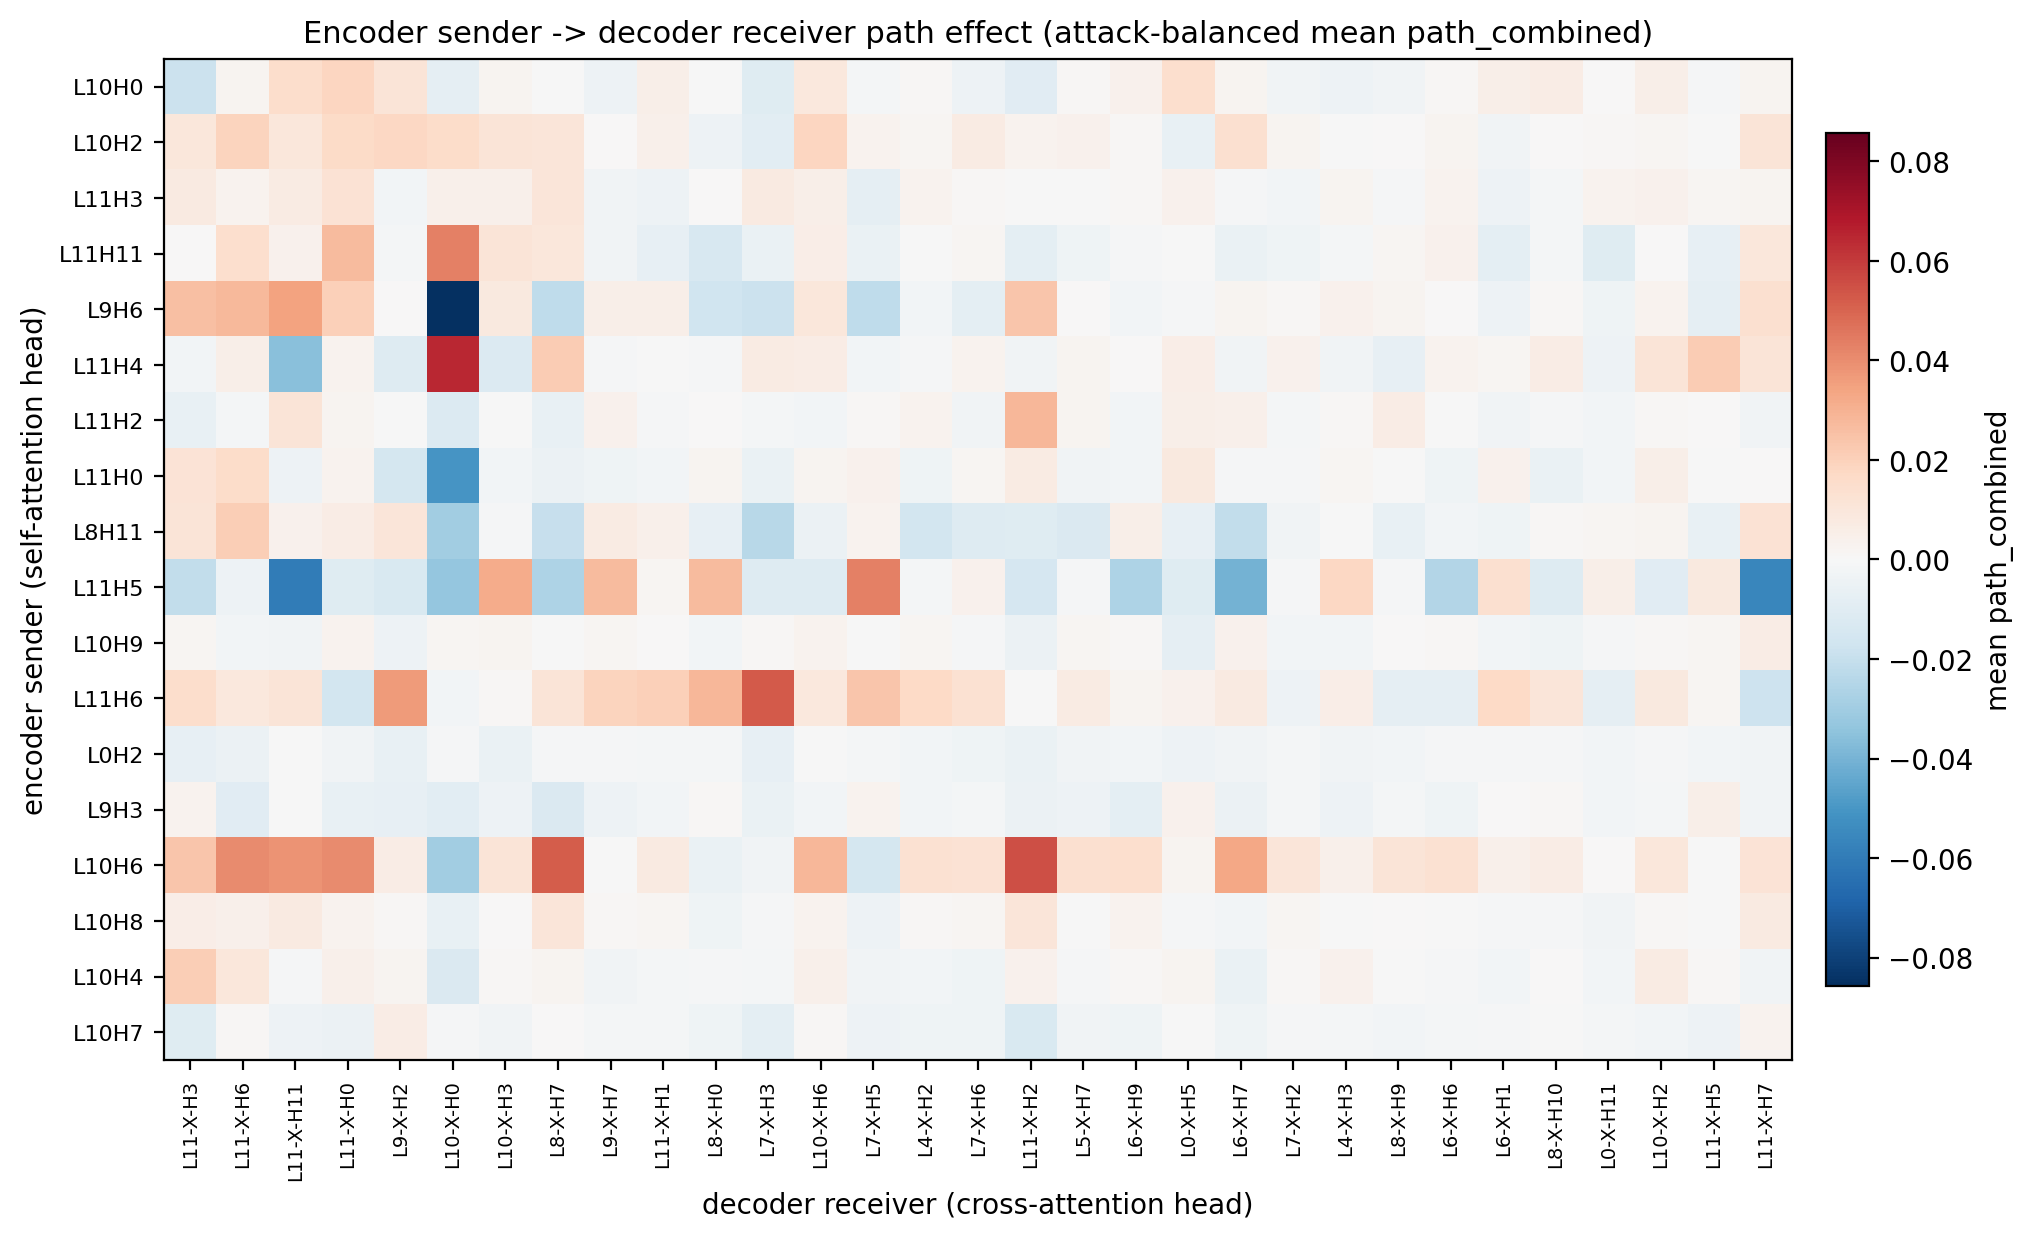
\includegraphics[width=0.95\textwidth]{outputs/plots/path_heatmap_combined.png}
  \caption{Attack-balanced mean $\pcomb$, 18 encoder senders (rows, architectural
  order) $\times$ 31 decoder receivers (columns, architectural order). No row
  or column is uniformly one colour — contrast the single dark cell
  \texttt{L9H6}$\to$\texttt{L10-X-H0} (most negative, $-0.086$) against the
  single bright cell \texttt{L11H4}$\to$\texttt{L10-X-H0} (most positive,
  $+0.065$) in the \emph{same column}: the pathway is not organised into
  senders or receivers that are simply ``good'' or ``bad'' routes, but into
  specific, sign-dependent pairs.}
  \label{fig:heatmap}
\end{figure}

\textbf{Prediction, stated before aggregating}: because every one of the 558
paths connects two independently-established causally-important heads
(Experiment 11's 18 and Experiment 3's 31), path patching should recover a
predominantly positive, non-trivial-magnitude picture. \textbf{Result: the
prediction does not hold.} The attack-balanced $\pcomb$ distribution across
558 pairs has mean $0.00093$ and \textbf{median $-0.00022$} (negative), std
$0.0122$, range $[-0.0856, +0.0647]$ — centered on zero, not displaced toward
positive values. \textbf{272 of 558 pairs (48.7\%) are positive, 286 (51.3\%)
are negative}, close to what an unbiased coin flip would produce. This is not
a failure to find signal: 20 pairs are positive on more than 80\% of the 105
attacks (a genuinely consistent effect, Section~\ref{sec:stability}), and the
single strongest paths reach $\pcomb \approx 0.06$--$0.09$, comparable in
magnitude to several of Experiment 11's own flagged encoder heads
(Table~\ref{tab:top10} there ranges 0.027--0.182). But the \emph{typical}
path, even between two independently-important endpoints, carries no
detectable attack-specific signal on its own — head importance and
head-to-head connectivity are measurably different claims, not two views of
the same fact.

The pathway is also diffuse rather than concentrated: of the 272 positive
pairs, the top 5 capture only 11.8\% of total positive path mass, and the top
50 (18\% of all positive pairs) capture 57.7\%. Unlike Experiments 11/3's own
sparse single-endpoint results (18/144, $\approx$22/288), no small clique of
pairs dominates the picture.

\begin{table}[H]
\centering
\caption{Top 10 paths by attack-balanced mean $\pcomb$ (all 105 attacks).
Stability = fraction of the 105 attacks with positive per-attack mean
$\pcomb$ for that pair.}
\label{tab:top10}
\begin{tabular}{llrrrr}
\toprule
Sender & Receiver & $\pcomb$ & $\pfwd$ & $\prev$ & Stability \\
\midrule
L11H4  & L10-X-H0  & 0.0647 & 0.0709 & 0.0695 & 78.1\% \\
L10H6  & L11-X-H2  & 0.0549 & 0.0685 & 0.0636 & 73.3\% \\
L11H6  & L7-X-H3   & 0.0522 & 0.0544 & 0.0558 & 85.7\% \\
L10H6  & L8-X-H7   & 0.0516 & 0.0600 & 0.0615 & 75.2\% \\
L11H11 & L10-X-H0  & 0.0434 & 0.0458 & 0.0462 & 61.9\% \\
L11H5  & L7-X-H5   & 0.0434 & 0.0452 & 0.0462 & 81.9\% \\
L10H6  & L11-X-H6  & 0.0405 & 0.0472 & 0.0454 & 86.7\% \\
L10H6  & L11-X-H0  & 0.0404 & 0.0448 & 0.0456 & 89.5\% \\
L10H6  & L11-X-H11 & 0.0383 & 0.0477 & 0.0458 & 85.7\% \\
L11H6  & L9-X-H2   & 0.0366 & 0.0428 & 0.0409 & 70.5\% \\
\bottomrule
\end{tabular}
\end{table}

\subsection{Forward and reverse mostly agree, but looser than single-unit patching}

\begin{figure}[H]
  \centering
  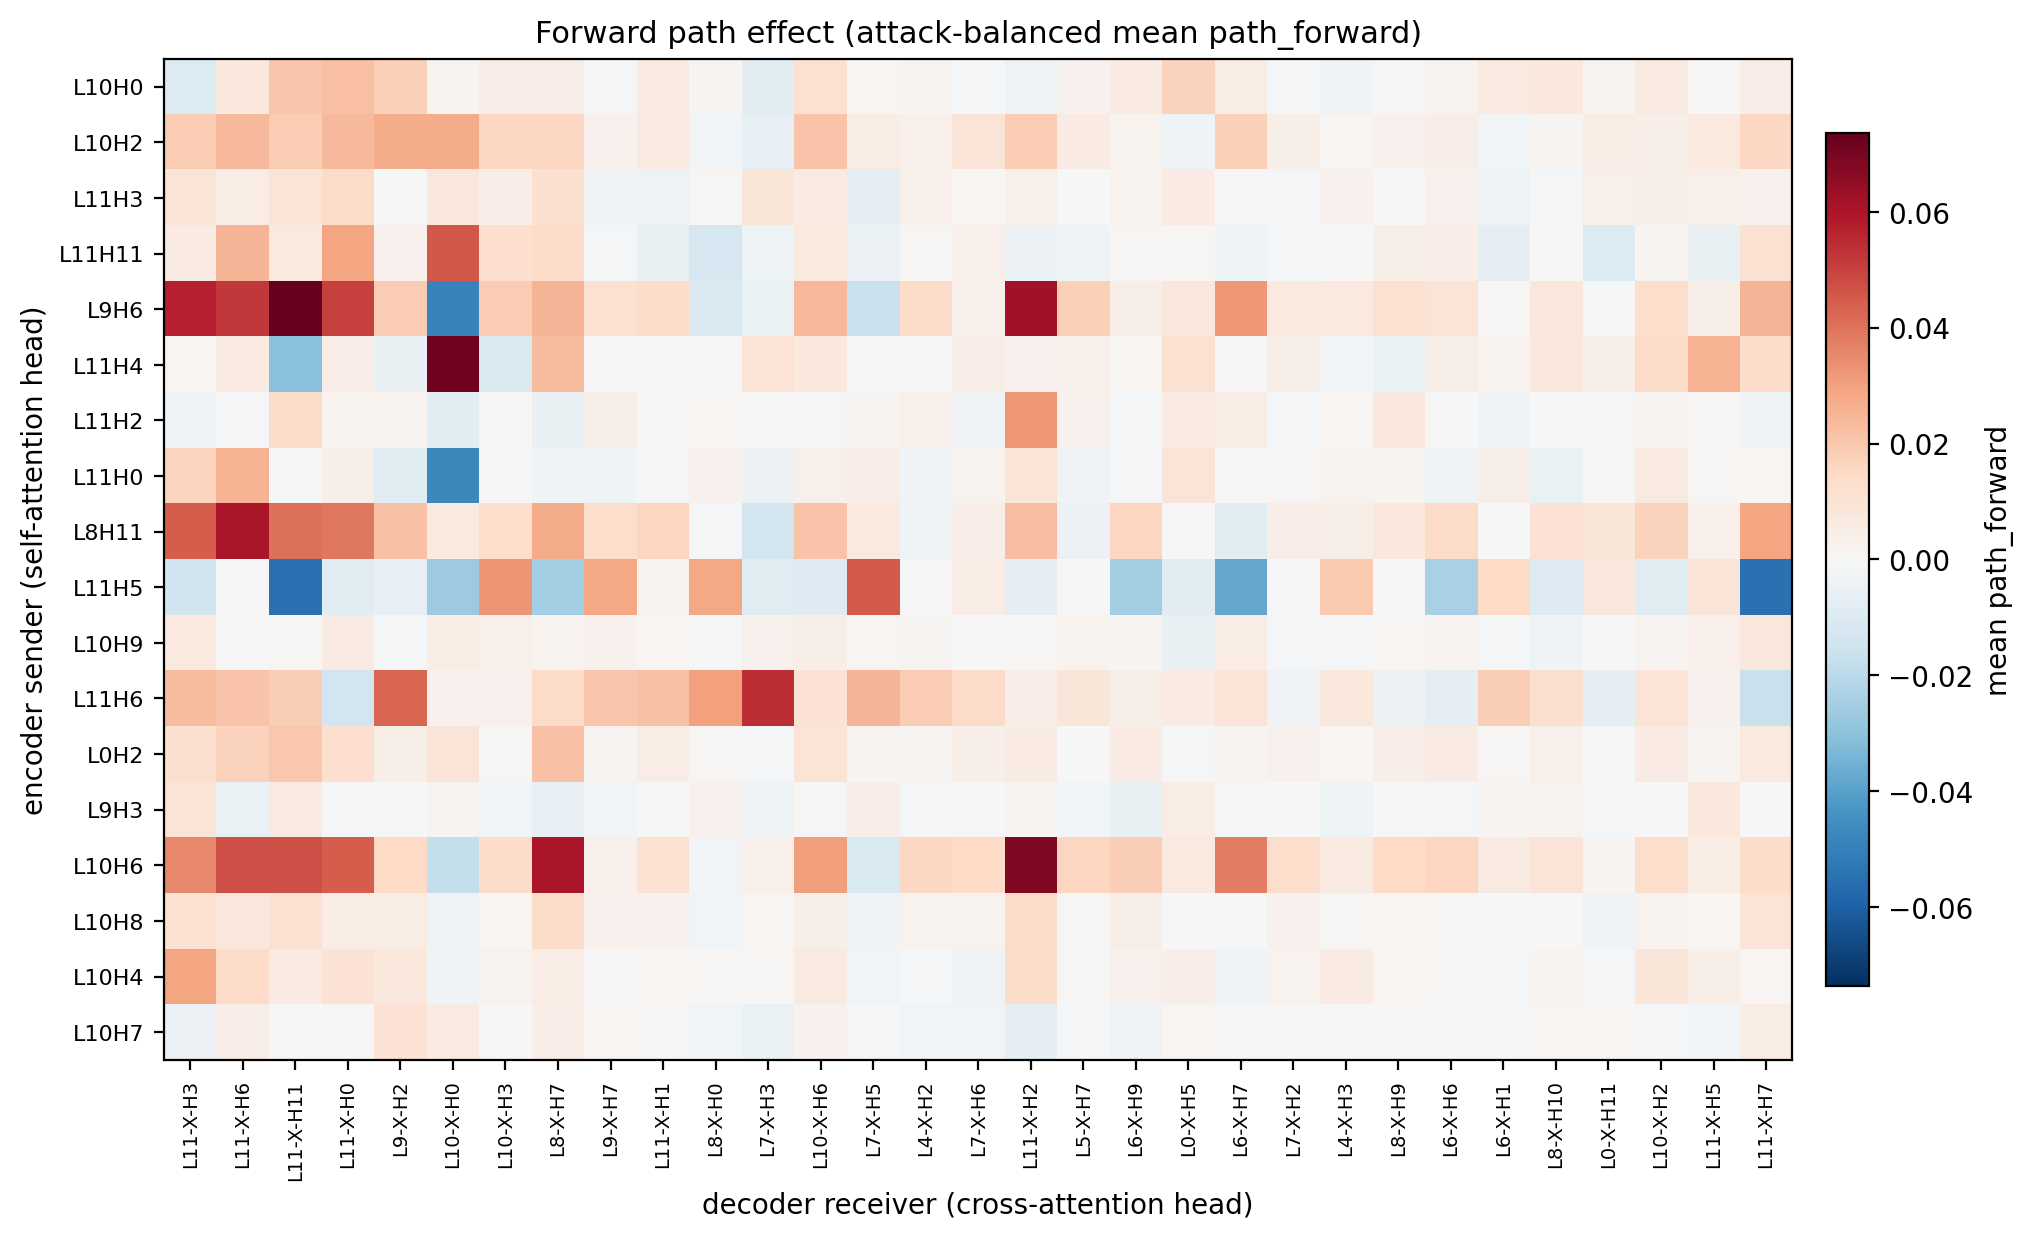
\includegraphics[width=0.95\textwidth]{outputs/plots/path_heatmap_forward.png}
  \caption{Attack-balanced mean $\pfwd$ (sufficiency: does injecting the
  isolated hybrid signal alone recover score?). Visually near-identical to
  Figure~\ref{fig:heatmap} — see Figure~\ref{fig:reverse} for the reverse
  (necessity) matrix and the quantitative agreement below.}
  \label{fig:forward}
\end{figure}

\begin{figure}[H]
  \centering
  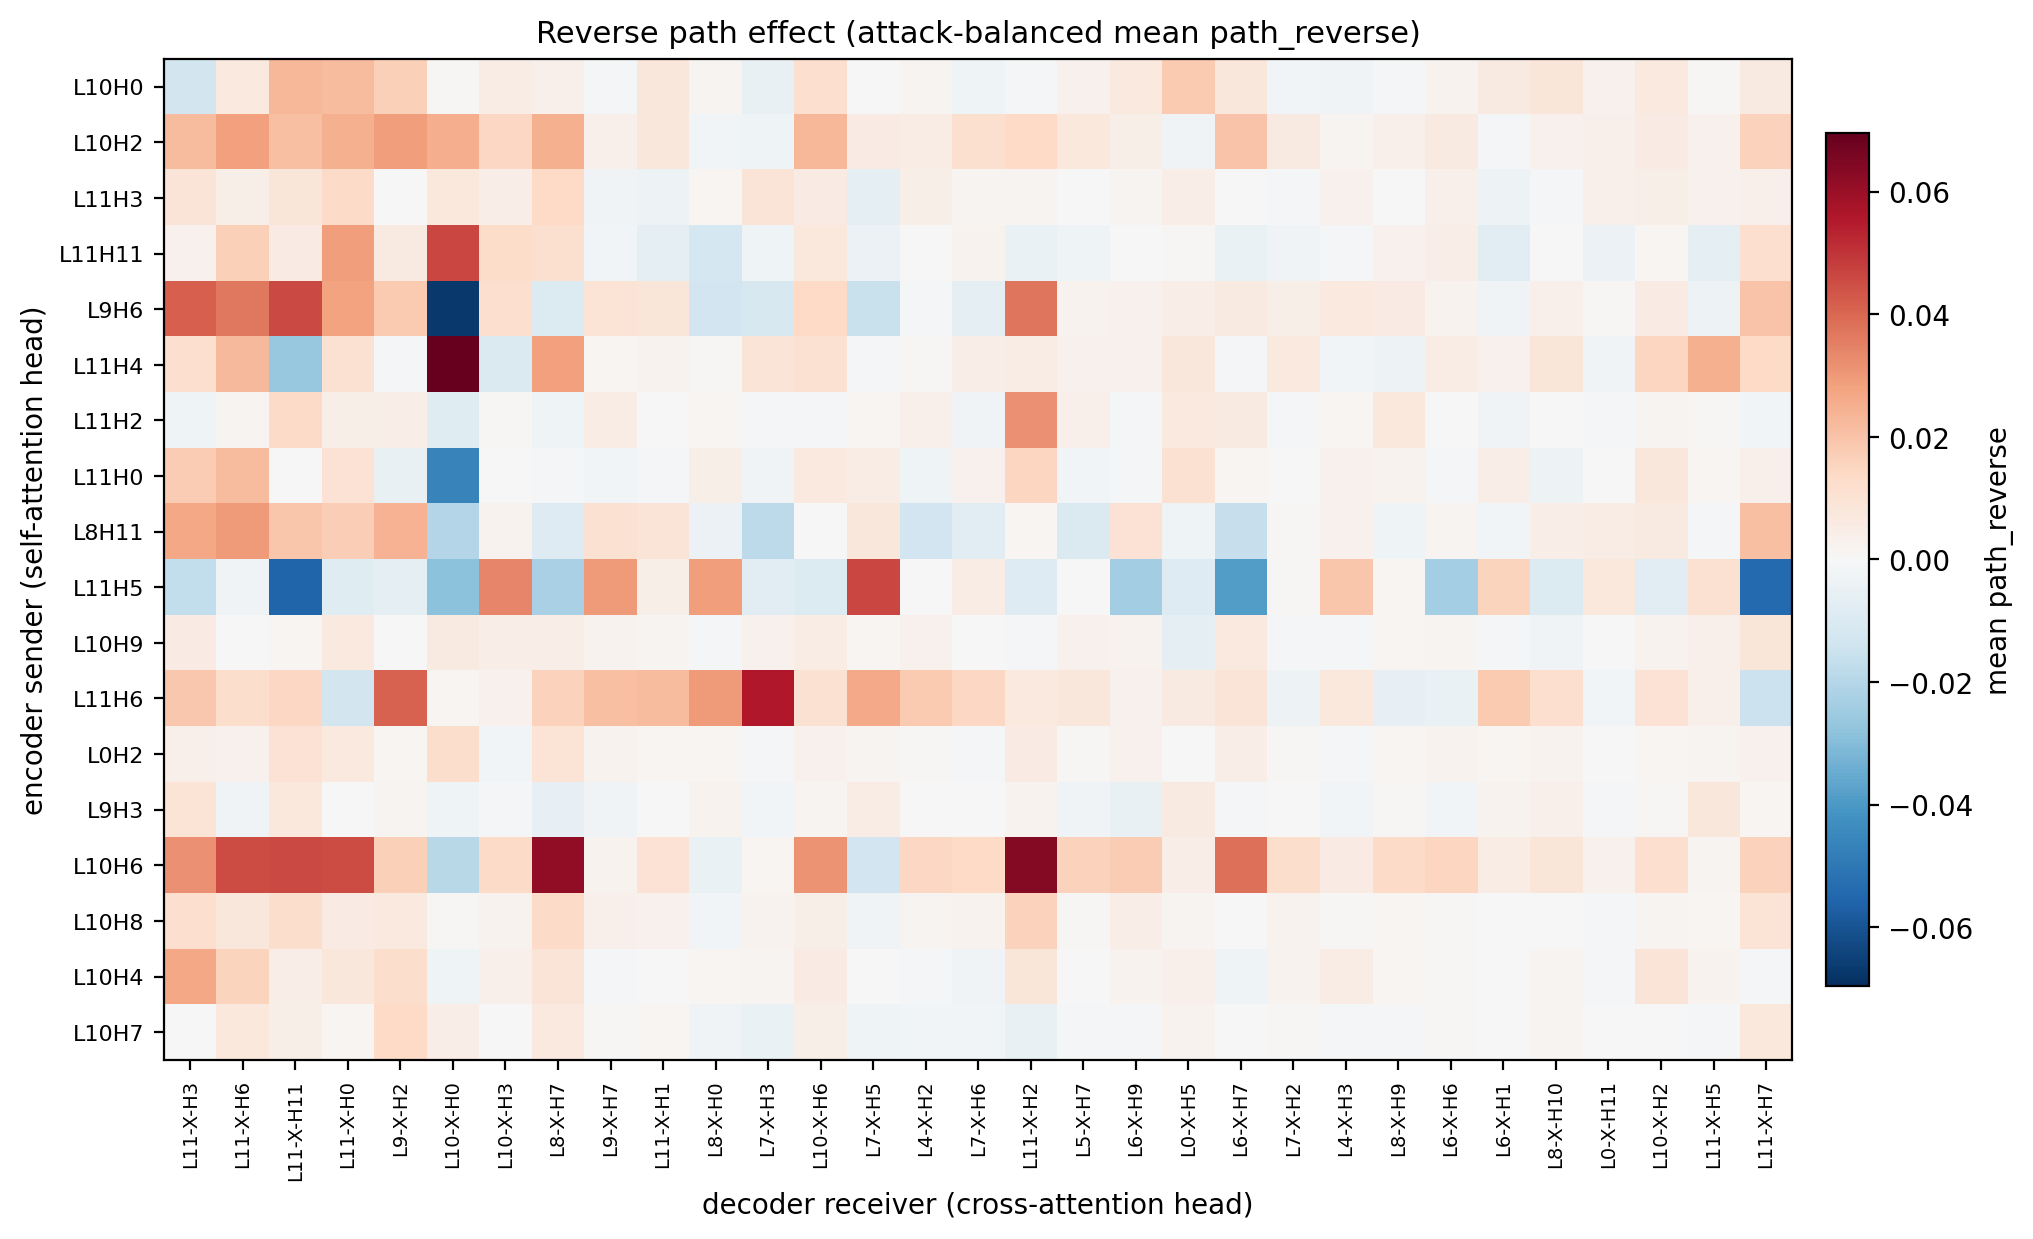
\includegraphics[width=0.95\textwidth]{outputs/plots/path_heatmap_reverse.png}
  \caption{Attack-balanced mean $\prev$ (necessity: does removing the
  isolated signal alone cancel score). Compare cell-by-cell against
  Figure~\ref{fig:forward}; the largest single forward/reverse gap in the
  whole matrix is \texttt{L8H11}$\to$\texttt{L8-X-H7} ($|\pfwd-\prev| = 0.036$),
  still small relative to the matrix's own dynamic range ($\approx$0.15).}
  \label{fig:reverse}
\end{figure}

Across all 558 pairs, Pearson $r(\pfwd, \prev) = 0.932$ and mean
$|\pfwd - \prev| = 0.0023$: where an isolated route is sufficient to move the
score, it is also close to necessary, and vice versa. This is the same
qualitative pattern Experiments 3 and 11 found for single-endpoint patching,
but quantitatively looser — Experiment 3's decoder heads showed mean
$|\fwd-\rev| \approx 0.0003$, roughly 7$\times$ tighter than here. Isolating a
two-endpoint route evidently introduces more forward/reverse asymmetry than
patching either endpoint alone, though not enough to change the qualitative
conclusion that sufficiency and necessity track each other closely for this
mechanism.

\subsection{A sign-split concentrated on one receiver: \texttt{L10-X-H0}}
\label{sec:split}

The single largest positive path and the single largest negative path in the
\emph{entire} $558$-pair matrix both terminate at the same receiver,
\texttt{L10-X-H0} (Table~\ref{tab:l10x0}). Of its 18 incoming sender paths,
only 4 are clearly positive and 14 are negative or negligible; the receiver's
own aggregate mean across all 18 senders is $-0.0084$ (the single worst
receiver in the receiver summary), yet its single best incoming path
(\texttt{L11H4}, $+0.0647$) is the single best path anywhere in the matrix.
\texttt{L10-X-H0} is not a uniformly weak receiver — it is a receiver whose
sign depends almost entirely on which encoder head is sending.

\begin{table}[H]
\centering
\caption{Receiver \texttt{L10-X-H0}: 4 strongest positive and 4 strongest
negative incoming sender paths (of 18 senders total; full breakdown in
\texttt{outputs/aggregates/global\_sender\_receiver\_long.csv}).}
\label{tab:l10x0}
\begin{tabular}{lrr}
\toprule
Sender & $\pcomb$ & Stability (fraction attacks positive) \\
\midrule
L11H4  & $+0.0647$ & 78.1\% \\
L11H11 & $+0.0434$ & 61.9\% \\
L10H2  & $+0.0157$ & 72.4\% \\
L11H3  & $+0.0041$ & 51.4\% \\
\midrule
L11H0  & $-0.0508$ & 31.4\% (i.e.\ negative on 68.6\%) \\
L10H6  & $-0.0296$ & 28.6\% \\
L11H5  & $-0.0330$ & 58.1\% \\
L9H6   & $-0.0856$ & 28.6\% (i.e.\ negative on 71.4\%) \\
\bottomrule
\end{tabular}
\end{table}

A second, smaller-scale split: \texttt{L0H2} is the only one of the 18
senders with \textbf{zero} of its 31 receivers positive — every single path
out of it is (weakly) negative, from $-0.0005$ to $-0.0070$. Unlike
\texttt{L10-X-H0}'s split, this is a uniform, if small, null-to-negative
result across the board for one specific early-layer head, not a
sender-dependent sign flip.

\subsection{Mean vs.\ median: outlier attacks inflate the headline pairs}

Every top-10 pair in Table~\ref{tab:top10} has an across-attack mean 2--3$\times$
its median: \texttt{L11H4}$\to$\texttt{L10-X-H0} has mean $0.0647$ but median
$0.0267$; \texttt{L9H6}$\to$\texttt{L10-X-H0} (the most negative pair) has
mean $-0.0856$ but median $-0.0229$. Per-attack values for the single
strongest pair range from $-0.42$ on \texttt{relevant\_end\_1} to $+0.99$ on
\texttt{false\_end\_3} — a handful of extreme attacks pull the mean well away
from the typical attack's effect. This is the same mean/median-disagreement
pattern Experiment 11 flagged for \texttt{L1-X-H7} ($-0.107$ mean vs.\
$-0.012$ median, driven by \texttt{bar\_random\_4}); it recurs here at the
path level and should be read the same way — the headline number describes
the average, not the typical, attack.

\begin{figure}[H]
  \centering
  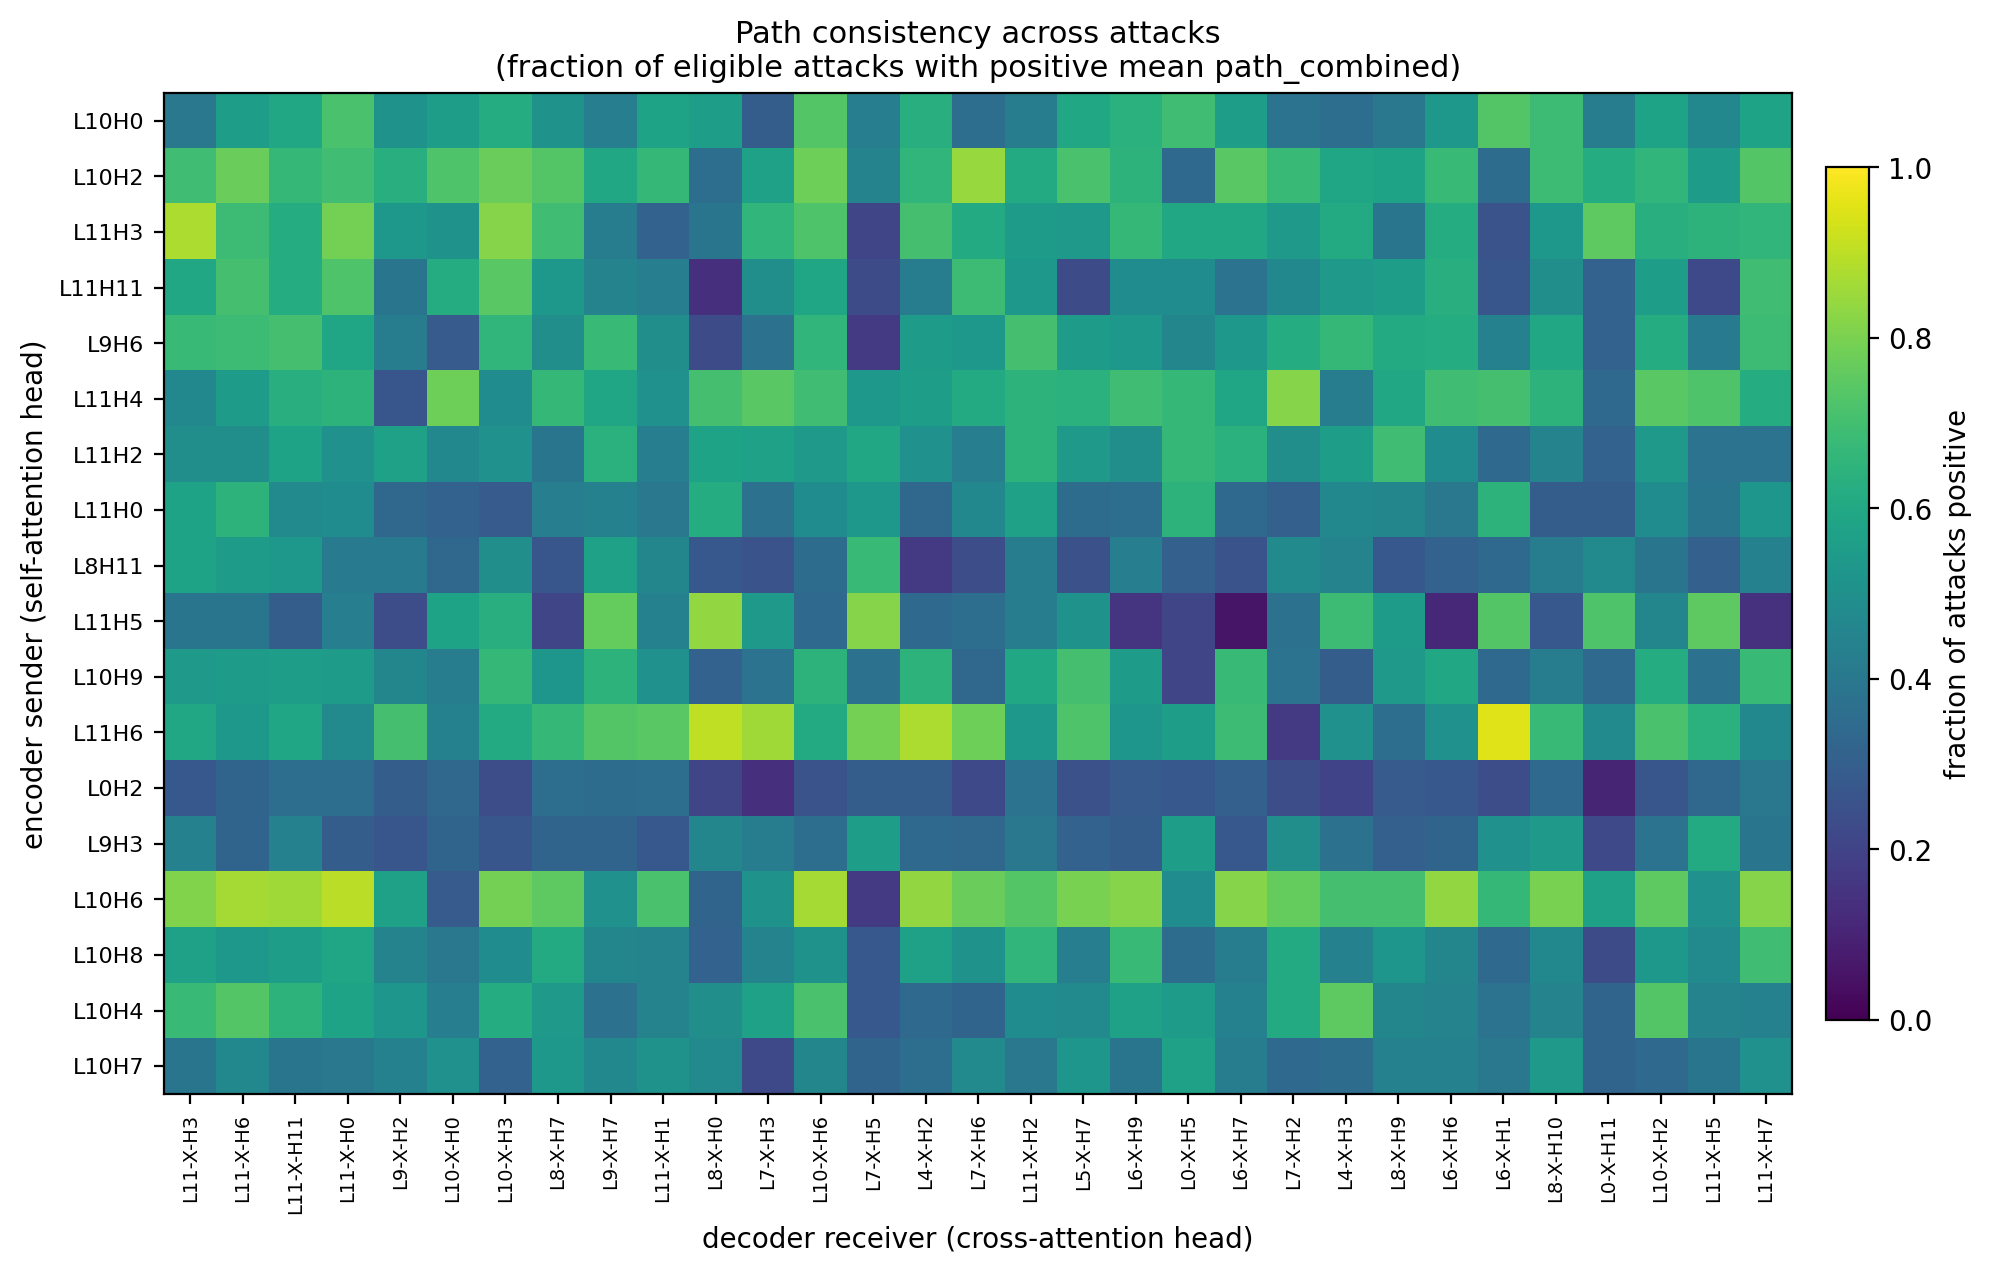
\includegraphics[width=0.75\textwidth]{outputs/plots/path_stability.png}
  \caption{Fraction of the 105 attacks with positive mean $\pcomb$, per
  pair. Note this is a \emph{separate} axis from Figure~\ref{fig:heatmap}'s
  magnitude — a pair can be highly consistent (stable near 0 or near 1) while
  still having small mean magnitude, and vice versa; the two figures should
  be read together, not one in place of the other.}
  \label{fig:stability}
\end{figure}

\subsection{Stability: 20 pairs are consistent, most are not}
\label{sec:stability}

Only \textbf{20 of 558 pairs (3.6\%)} are positive on more than 80\% of the
105 attacks; \textbf{11 pairs (2.0\%)} are negative on more than 80\% of
attacks. The remaining $\sim$94\% sit closer to chance-level consistency
(285/558, or 51.1\%, are positive on a bare majority, $>$50\%, of attacks) —
consistent with the near-zero, symmetric overall distribution in
Section~\ref{sec:diffuse}. The most consistent pairs
(\texttt{L11H6}$\to$\texttt{L6-X-H1} at 95.2\%, \texttt{L11H6}$\to$\texttt{L8-X-H0}
at 90.5\%, \texttt{L10H6}$\to$\texttt{L11-X-H0} at 89.5\%) are not the same
pairs as the largest-magnitude ones in Table~\ref{tab:top10} — a genuinely
consistent small effect and a genuinely large but outlier-driven effect are
different findings, and neither implies the other.

\subsection{Standalone importance does not predict path-connectivity rank}

\textbf{Prediction, stated before computing}: since both head sets were
selected \emph{because} they matter individually, a head's standalone
importance rank (Experiment 11's canonical ranking for senders, Experiment
3's Grid~A ranking for receivers) should predict its rank in this
experiment's path-connectivity summary (mean path effect across its 31 or 18
counterparts). \textbf{Result: the prediction does not hold for senders and
holds only weakly for receivers.} Sender standalone rank vs.\ path-connectivity
rank: Spearman $\rho = 0.259$, $p = 0.30$ — not distinguishable from no
correlation. The single most important standalone sender, \texttt{L10H0}
(canonical $\comb = 0.182$, rank 1/18), falls to \textbf{rank 8/18} in mean
path effect ($0.0012$, barely positive); the strongest path-connectivity
sender, \texttt{L10H6} (mean path effect $0.0132$, positive on 25/31
receivers), ranked only \textbf{15/18} standalone ($0.031$, barely over the
flag threshold). Receiver standalone rank vs.\ path-connectivity rank:
Spearman $\rho = 0.450$, $p = 0.011$ — weak but statistically significant,
the one place the prediction partially survives. \texttt{L11-X-H3}, the
single strongest standalone receiver ($\comb = 0.082$, rank 1/31), stays
reasonably high at path-rank 4/31; but \texttt{L10-X-H0} (standalone rank
6/31, $\comb = 0.038$) is \textbf{dead last, 31/31}, by path-connectivity
mean, for the reasons detailed in Section~\ref{sec:split}.

\subsection{Super-additivity recurs at the individual-path level}

Several individual paths exceed \emph{either endpoint's own full-network
standalone effect} — a path between two heads is, by itself, a stronger
signal than either head's aggregate single-endpoint importance measurement.
\texttt{L10H6}$\to$\texttt{L11-X-H2} ($\pcomb = 0.0549$) is $1.77\times$
\texttt{L10H6}'s own standalone canonical effect ($0.0311$) and $2.49\times$
\texttt{L11-X-H2}'s own standalone Grid~A effect ($0.0221$);
\texttt{L11H6}$\to$\texttt{L7-X-H3} is $1.47\times$/$2.04\times$; the top
path overall, \texttt{L11H4}$\to$\texttt{L10-X-H0}, is $0.89\times$ the
sender's standalone effect and $1.69\times$ the receiver's. This is the same
qualitative phenomenon Experiment 11's Step 3 reported for whole-layer vs.\
summed-single-head effects ($1.76\times$, super-additive, contradicting a
sub-additive prediction): different interventions (single-endpoint full-network
patch vs.\ two-endpoint isolated-route patch) are not nested subsets of one
another, so a route's isolated effect can exceed what either endpoint's own
standalone measurement would suggest is available. This is not a
contradiction in the data; it is evidence that these heads' contributions
interact rather than sum independently, at both the whole-layer granularity
Experiment 11 examined and the individual-path granularity examined here.

\begin{figure}[H]
  \centering
  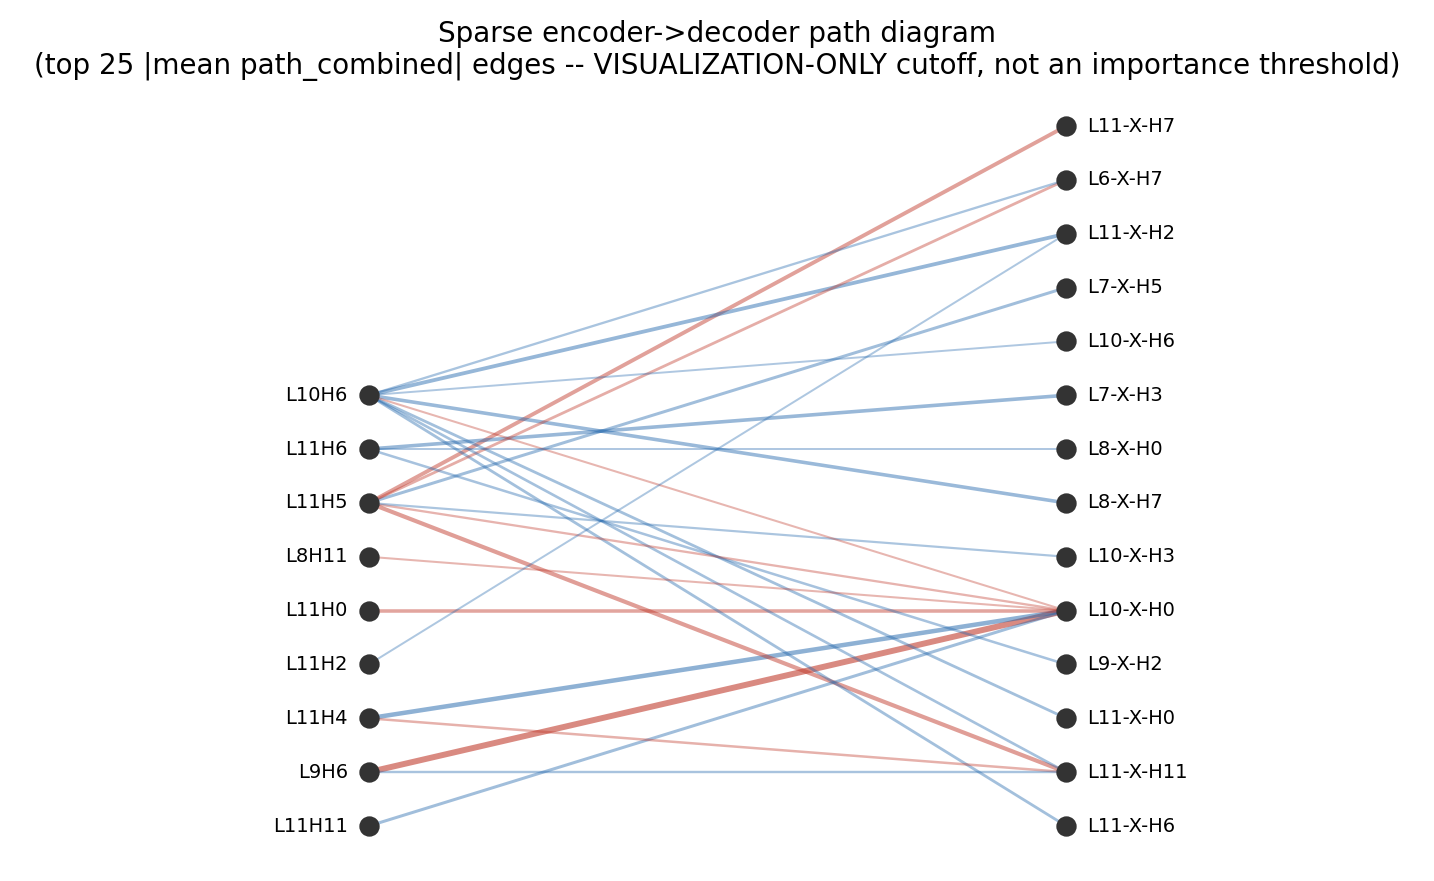
\includegraphics[width=0.8\textwidth]{outputs/plots/sparse_circuit_topk.png}
  \caption{Diagnostic-only network view of the top 25 $|\pcomb|$ edges (a
  visualization cutoff, not an importance threshold — see
  Section~\ref{sec:diffuse}'s concentration numbers for why a much larger set
  of pairs than 25 carries meaningful, if smaller, signal). Edge colour
  encodes sign (blue positive, red negative); \texttt{L10-X-H0}'s dual role
  from Section~\ref{sec:split} is visible as both a strong blue and a strong
  red edge converging on the same node.}
  \label{fig:sparse}
\end{figure}

% =====================================================================
\section{Overall Interpretation and Discussion}
% =====================================================================

\begin{enumerate}
  \item \textbf{Head importance and head-to-head connectivity are different
  claims, and the numbers show it.} 558 paths between two independently
  causally-important head sets split almost exactly down the middle
  (48.7\%/51.3\% positive/negative) with a slightly negative median — the
  natural prediction that both-important implies mostly-positive-route does
  not hold. Sections 4.5 and 4.6 are each individually correct; neither
  implies the other's heads are connected in the way a reader might assume.
  \item \textbf{The pathway is diffuse, not a sparse circuit.} No small
  clique of pairs dominates (top 50 of 272 positive pairs capture 57.7\% of
  positive mass); this contrasts with both endpoint experiments' own sparse
  single-unit results and means a defense or explanation strategy cannot
  target ``the'' encoder-to-decoder route — there are many small ones.
  \item \textbf{One receiver, \texttt{L10-X-H0}, carries both the single
  strongest and (via a different sender) an extremely negative path, while
  being the worst receiver on aggregate.} Standalone importance measurements
  (Experiment 3) would rank it 6th; path-connectivity analysis reveals it is
  actually a sign-split, sender-dependent node, not a moderately-important
  uniform one — this distinction is invisible to single-endpoint patching by
  construction.
  \item \textbf{Standalone rank is a weak-to-absent predictor of
  path-connectivity rank.} Not significant for senders ($\rho=0.259$),
  weakly significant for receivers ($\rho=0.450$). Selecting heads for a
  path-patching study by their own single-endpoint importance is a reasonable
  starting scope (as this experiment did, per the task design), but their
  standalone ranking should not be used to predict which specific pairs will
  turn out to matter.
  \item \textbf{Super-additivity is not an isolated Experiment-11 finding —
  it recurs at finer granularity.} Individual paths exceeding either
  endpoint's own full-network effect (up to $2.49\times$) confirms these
  heads' contributions genuinely interact rather than sum, at both the
  whole-layer and individual-path scale; any future additive combination
  search (Phase 4-style) needs to measure combined effects directly rather
  than infer them from single-unit or single-path numbers.
  \item \textbf{Where an effect exists, it behaves like the ones found
  before it.} Forward/reverse agreement ($r=0.93$) and the mean/median
  outlier-attack pattern both reproduce Experiments 3/11's qualitative
  findings, just measured at a looser tolerance for the two-endpoint
  intervention — the underlying mechanism-validation logic transfers, even
  though the headline connectivity story does not.
\end{enumerate}

% =====================================================================
\section{Limitations and Threats to Validity}
% =====================================================================

\begin{itemize}
  \item \textbf{Coarse sender position only.} Sender $A$ is patched at all
  encoder positions at once; no restriction to query-word, document, or
  attack-token positions. Token-specific path patching, combining this
  experiment's strongest/stablest pairs with Experiment 1's query-token
  localisation, is explicitly deferred to Experiment 2B.
  \item \textbf{31-receiver set is rank-based, not the report-stated
  threshold set.} Experiment 3's report claims a threshold-based 31-head
  cross-attention set that does not reproduce from any on-disk aggregate
  (Methodology Step 1); this experiment substitutes a top-31-by-rank set
  from the same underlying data, a documented and reproducible but
  \emph{different} selection rule than the one the report describes.
  \item \textbf{No importance threshold applied to the path matrix.} Per
  task design, all continuous $\pcomb$ values are reported as-is; ``diffuse,''
  ``sparse,'' and ``consistent'' above are descriptive characterisations of
  the distribution (concentration ratios, positive/negative counts,
  stability fractions), not a newly-invented cutoff for calling a specific
  pair important.
  \item \textbf{Up to 10 examples/attack.} The initial breadth pass; the
  pipeline is built to rerun unchanged at $n{=}30$ or $n{=}100$ (only
  \texttt{run.max\_examples\_per\_attack} in \texttt{configs/default.yaml}
  changes), which would tighten the per-attack means and could shift some
  borderline pairs (Section~\ref{sec:stability}'s 51\%-consistent middle
  group is the most likely to move).
  \item \textbf{Single model/dataset.} Results are for monoT5-base on DL19,
  matching every prior experiment in this project.
\end{itemize}

% =====================================================================
\section{Reproducibility}
% =====================================================================

From \texttt{13\_monot5\_encoder\_decoder\_path\_patching/}, with the
\texttt{advseq2seq} conda environment and Experiments 1, 3, and 11's outputs
present as sibling directories:

\begin{lstlisting}
bash bash/run_debug.sh                     # debug run + all 8 sanity checks
bash bash/run_sweep.sh configs/default.yaml   # full sweep + aggregate + plots (resume-safe)
bash bash/run_sweep.sh --max-examples 30      # later n=30 pass, same config, no code changes
\end{lstlisting}

\noindent On this run: SLURM job 1280967, 1$\times$ L40 GPU, $\approx$2h48m
wall-clock for the full 105-attack $\times$ 10-example $\times$ 558-path
sweep plus aggregation and plots; outputs under
\texttt{outputs/\{raw,aggregates,plots,diagnostics\}/}, exact sender/receiver
head lists in \texttt{configs/heads/*.json}, and the sanity-check report in
\texttt{outputs/diagnostics/sanity\_check\_report.txt}.

% =====================================================================
\section*{Appendix: Glossary of Key Quantities}
\addcontentsline{toc}{section}{Appendix: Glossary of Key Quantities}
% =====================================================================

\begin{description}[leftmargin=1.8em,style=nextline]
  \item[path] one (sender encoder head $A$, receiver decoder cross-attention
  head $B$) pair; 558 total ($18 \times 31$).
  \item[$\pfwd$ / $\prev$ / $\pcomb$] forward/reverse/combined \emph{path}
  effect (Eqs.~\ref{eq:pfwd}--\ref{eq:pcomb}), the two-endpoint generalisation
  of Experiments 1/3/11's single-endpoint $\fwd/\rev/\comb$.
  \item[hybrid encoder representation] the base run's own encoder
  computation with sender $A$'s activation spliced in from the other run,
  propagated normally through the remaining encoder layers.
  \item[attack-balanced aggregation] average of per-attack means (not a flat
  average over all examples), so an attack with more qualifying examples
  does not dominate the global summary merely by row count.
  \item[stability] fraction of the 105 attacks whose per-attack mean
  $\pcomb$ for a given pair is positive.
  \item[standalone effect] a head's own single-endpoint $\comb$ from
  Experiment 11 (senders, canonical attack) or Experiment 3 (receivers,
  Grid~A), i.e.\ the importance measurement this experiment's head sets were
  selected by.
\end{description}

\end{document}
